\documentclass[a4paper, 12pt]{article}
\usepackage[margin=1in]{geometry}
\usepackage{graphicx}
\geometry{left=1in, right=1in, top=1in, bottom=1in}

\title{Audio Features Workshop 2024}
\author{Honnavalli Pranaav \\ 3905020}
\date{}

\begin{document}

\maketitle

\section*{Assignment 1 - BPM Estimation}
For the Kevin MacLeod track,
By listening to the beat, the BPM is estimated to \textbf{115bpm}
By calculating using librosa, the estimated BPM is: \textbf{129.2bpm}
\newline
For the track01ErosRamazotti.mp3,
By listening to the beat, the BPM is estimated to \textbf{84bpm}
By calculating using librosa, the estimated BPM is: \textbf{61.25bpm}

\section*{Assignment 2 - Harmonic Percussive Sound Seperation}
\begin{figure}[h!]
    \centering
    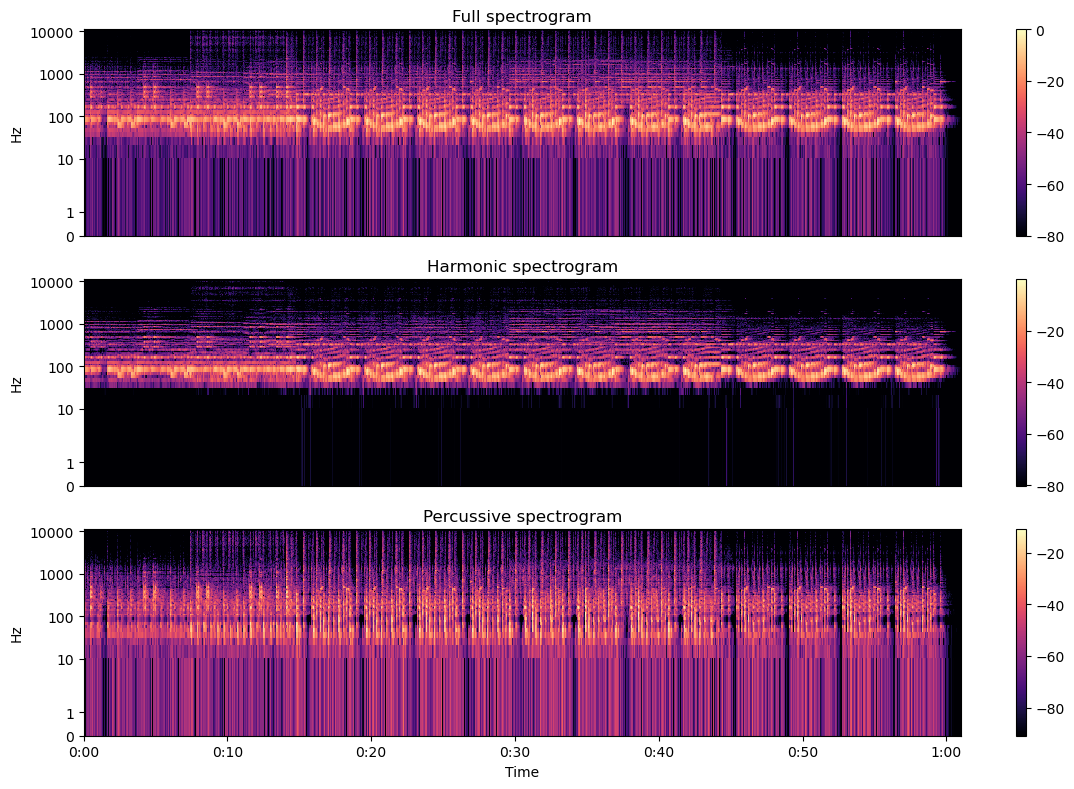
\includegraphics[width=0.8\textwidth]{./images/hprss-mcleod-output.png}
    \caption{Harmonic Percussive Sound Separation Kevin McLeod}
    \label{fig:hpssmcleod}
\end{figure}

\begin{figure}[h!]
    \centering
    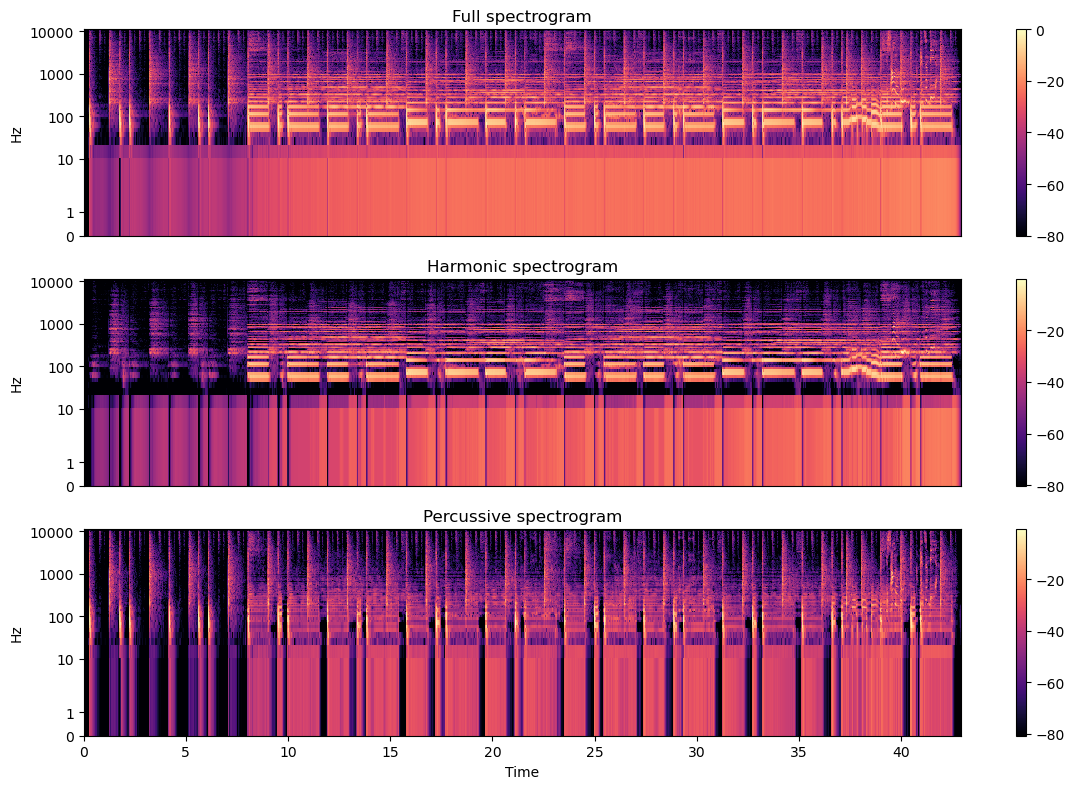
\includegraphics[width=0.8\textwidth]{./images/hprss-track01-output.png}
    \caption{Harmonic Percussive Sound Separation Eros Ramazotti}
    \label{fig:hpsseros}
\end{figure}

From the 2 plots (Figure~\ref{fig:hpsseros} and Figure~\ref{fig:hpssmcleod}), we can see that the percussive spectogram has more defined peaks at regular intervals from which one may be able to estimate the bpm. The 
harmonic spectogram is more continuous. We see that for a high bpm sound like the Kevin McLeod track, the percussive spectogram shows and increase in the 
defined energy spikes as compared to the lower bpm Eros Ramazotti (track01) track.
\newline

\begin{figure}[h!]
    \centering
    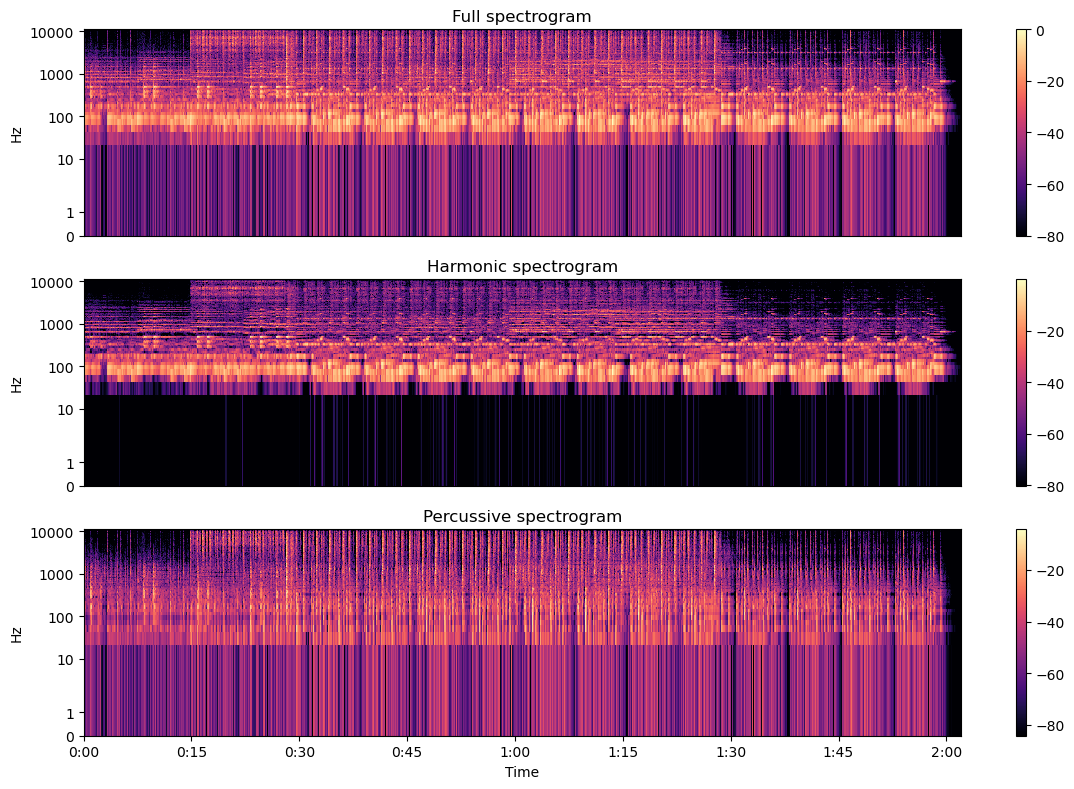
\includegraphics[width=0.8\textwidth]{./images/hprss-mcleod-output-custom.png}
    \caption{Harmonic Percussive Sound Separation Custom}
\label{fig:hpsstrack02}
\end{figure}
To get the above figure \ref{fig:hpsstrack02}, we first selected a lower nfft and hoplength values to better derive frequencies for percussive sounds which need better frequency resolution
as they occur in a small window. Next we add a filter (High-Pass), which eliminates any low frequency noise from the audio file data. Finally, we 
normalize the audio data to get clearer peaks for the percussive sounds. Another thing to be noted is that with an increase in margin, the percussive data is more 
visible in the spectogram.

\section*{Assignment 3}
\end{document}